%%%%%%%%%%%% Attribution %%%%%%%%%%%%
% This template was created by 
% Chuck F. Rocca at WCSU and may be
% copied and used freely for 
% non-commercial purposes.
% 10-17-2021
%%%%%%%%%%%%%%%%%%%%%%%%%%%%%%%%%%%%%

%%%%%%% Start Document Header %%%%%%%
% In creating a new document
% copy and paste the header 
% as is.
%%%%%%%%%%%%%%%%%%%%%%%%%%%%%%%%%%%%%

\documentclass{article}

%%%% Header Information %%%%
    %%% Document Settings %%%%
    \usepackage[utf8]{inputenc}
    \usepackage[
        twoside,
        top=1in,
        bottom=0.75in,
        inner=0.5in,
        outer=0.5in
    ]{geometry}
    \pagestyle{myheadings}

%%%% Additional Commands to Load %%%%
    \usepackage{tcolorbox}
    \tcbuselibrary{skins}
    \usepackage{minted}
    \usepackage{color}
    \usepackage{tikz}
    \usetikzlibrary{calc}
    \usepackage{tabularx,colortbl}
    \usepackage{amsfonts,amsmath,amssymb}
    \usepackage{titling}
    \usepackage{mathrsfs}
    \usepackage{calc}
    \usepackage{xepersian}

%%%% Commands to Define Homework Boxes %%%%
%%%% Box Definition %%%%
    \newtcolorbox{prob}[1]{
    % Set box style
        sidebyside,
        sidebyside align=bottom,
    % Dimensions and layout
        width=\textwidth,
        toptitle=2.5pt,
        bottomtitle=2.5pt,
        righthand width=0\textwidth,
    % Coloring
        colbacktitle=gray!30,
        coltitle=black,
        colback=white,
        colframe=white,
    % Title formatting
        title={
            #1 \hfill نمره:\phantom{WWWW}
        },
        fonttitle=\large\bfseries
    }

%%%% Environment Definition %%%%
    \newenvironment{problem}[1]{
        \begin{prob}{#1}
    }
    {
        \tcblower
        \centering
        \vspace{\baselineskip}
        \end{prob}
    }



%%%% Document Information %%%%
    \title{تکلیف سری دوم کنترل دیجیتال}
    \date{نیسمال دوم 1402-1403}
    \author{استاد درس : دکتر طالبی}

%%%%%%% End Document Header %%%%%%%


%%%% Begin Document %%%%
% note that the document starts with
% \begin{document} and ends with
% \end{document}
%%%%%%%%%%%%%%%%%%%%%%%%
\settextfont{BNAZANIN.TTF}

\begin{document}

%%%% Format Running Header %%%%%
\markboth{\theauthor}{\thetitle}

%%%% Insert the Title Information %%%
% \maketitle


%%%% General Description of the Document %%%%
\begin{figure}[htbp]
    \centering
    
\includegraphics[width=\linewidth]{Header.png}
    % \caption{Caption}
    % \label{fig:enter-label}
\end{figure}
\setlatintextfont{Feelfree Personal Use}

\centering
"\lr{Well done is better than well said.}"

\lr{-Benjamin Franklin}-

\setlatintextfont{Times New Roman}
\raggedleft
%%%% Introduction to the General Template %%%%
\section{بخش مقدماتی (35 نمره)}
\centering
حل \underline{دو سوال} از این بخش الزامی است.


    \begin{problem}{سوال اول}
    (تبدیل \lr{z}) به روش بسط کسر های جزئی تبدیل معکوس \lr{z} زیر را بدست آورید :
    
    \centering
    \lr{X(z) = $\frac{2z^3 + z}{(z-2)^3(z-1)}$}
    
    \end{problem}

    \begin{problem}{سوال دوم}
    	(تحقق) تابع تبدیل 
    	\lr{G(z)}
    	 را درنظر بگیرید.
    	 
    	 \centering
    	 $G(z) = \frac{z-2}{(z-0.1)(z^2-0.5z+1)}$
    	 
    	 \raggedright
	تحقق سری سیستم ذیل را بدست آورید (برای بلوک‌های سری از تحقق رؤیت پذیر استفاده نمایید)
    	 
    \end{problem}
    
    \begin{problem}{سوال سوم}
    	(نگهدار ها) نشان دهید مدار شکل زیر بصورت یک نگهدار مرتبه صفر عمل می‌کند.
    \end{problem}
    
    \begin{figure}[htbp]
    	\centering
    	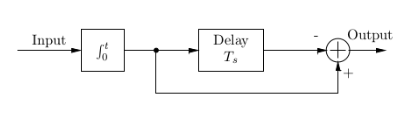
\includegraphics{Second Series/4.png}
    	\caption{شکل سوال سوم}
    \end{figure}
    
    
    \begin{problem}{سوال چهارم}
    	(نگهدار ها) دیاگرام بلوکی شکل زیر را در نظر بگیرید نشان دهید هرگاه سیگنالی با مقدار 1 در نقطه 0 و مقدار 0 در سایر نقاط (سیگنال ضربه گسسته) به عنوان ورودی به آن اعمال شود مانند نگهدار مرتبه اول عمل می‌کند. (خروجی را رسم کنید.)
    \end{problem}
    \begin{figure}[htbp]
    	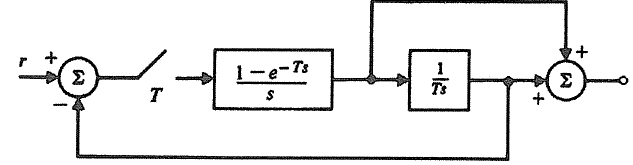
\includegraphics[width=\linewidth]{Second Series/5.png}
    	\caption{شکل سوال چهارم}
    \end{figure}
    
    \begin{problem}{سوال پنجم}
    	(تبدیل ستاره) تبدیل ستاره تابع تبدیل زیر را با روش دلخواه بدست آورید.
    	
    	\centering
    	$G(s) = \frac{s+2}{s(s+1)}$
    	
    	\raggedright
    \end{problem}
\raggedleft    
\section{بخش متوسط (35 نمره)}
\centering
حل \underline{دو سوال} از این بخش الزامی است.
\begin{problem}{سوال ششم}
	(تبدیل \lr{z}) با توجه به معادله تفاضلی زیر به سوالات پاسخ دهید.

\centering
$y(0) = y(1) = 0 , e(0) = 0 , e(k) = 1 , k = 1,2,...$


\lr{$y(k+2) - \frac{3}{4}y(k+1) + \frac{1}{8}y(k) = e(k)$}

\raggedright

الف) $y(k)$ را به صورت عددی برای
$0 \leq k \leq 4$
 بدست آورید.
  
  ب) آیا تابع تبدیل این سیستم پایدار است؟ استدلال کنید.

\end{problem}
	

\begin{problem}{سوال هفتم}
	(تحقق) تابع تبدیل زیر را در نظر بگیرید.
	
	\centering
	$D(z) = \frac{2z^2 - 2.4z + 0.72}{z^2 - 1.4z + 0.98}$
	
	\raggedright
	با توجه به شکل ضرایب مجهول را بدست آورید (مقصود از $T$ تاخیر است)
\end{problem}
\begin{figure}
	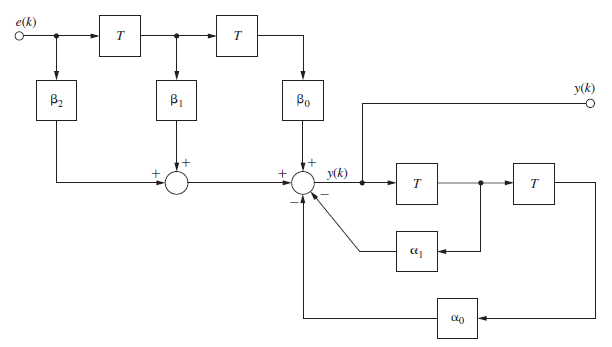
\includegraphics[width=\linewidth]{Second Series/2.png}
	\caption{شکل سوال هفتم}
\end{figure}

\begin{problem}{سوال هشتم}
	(تحقق) تابع تبدیل زیر را در نظر بگیرید.
	
	\centering
	$D(z) = \frac{2z^2 - 2.4z + 0.72}{z^2 - 1.4z + 0.98}$
	
	\raggedright
	با توجه به شکل ضرایب مجهول را بدست آورید (مقصود از $T$ تاخیر است)

\end{problem}
\begin{figure}
	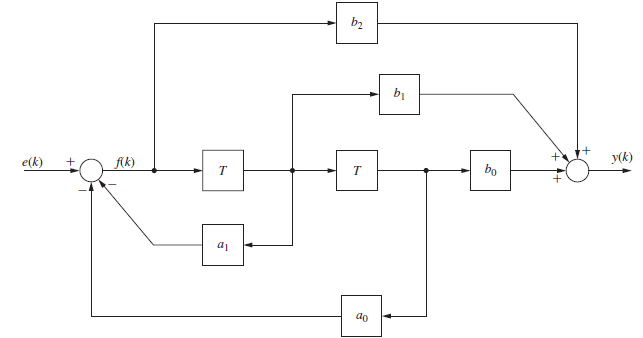
\includegraphics[width=\linewidth]{Second Series/3.png}
	\caption{شکل سوال هشتم}
\end{figure}


\begin{problem}{سوال نهم}
	(نگهدار ها) یک سیستم با تابع تبدیل زمان پیوسته‌ی
	\lr{G(s)}
	را در نظر بگیرید:
	
	\centering
	$G(s) = \frac{e^{-s}}{(s+1)(s+2)}$
	
	\raggedright
	با استفاده از نگهدار مرتبه صفر و 
	$T = 0.5$
	سیستم را نمونه برداری نمایید.
\end{problem}


\begin{problem}{سوال دهم}
	(تبدیل ستاره) الف) تبدیل ستاره را برای دو تابع زیر به ازای 
	$T = 0.1 s$
	بدست آورید توضیح دهید که چرا پاسخ آنها یکسان است؟
	
	\raggedleft
	$1) cos(4 \pi t)$
	
	$2) cos(16 \pi t)$
	
	\raggedright
	ب) تابع دیگری را معرفی کنید که تبدیل ستاره برابر با آنچه بدست آوردید داشته باشد
	
\end{problem}


\raggedleft
\section{ بخش تکمیلی (30 نمره)}
\centering
حل \underline{دو سوال} از این بخش الزامی است.
\begin{problem}{سوال یازدهم}
	(تبدیل \lr{z}) هر یک از توابع پالسی ذیل متناظر با پاسخهای پله‌ی
	\lr{A - F}
	 هستند. این تناظر را با ذکر دلیل و استدلال کامل مشخص کنید.
\end{problem}
\begin{figure}[htbp]
	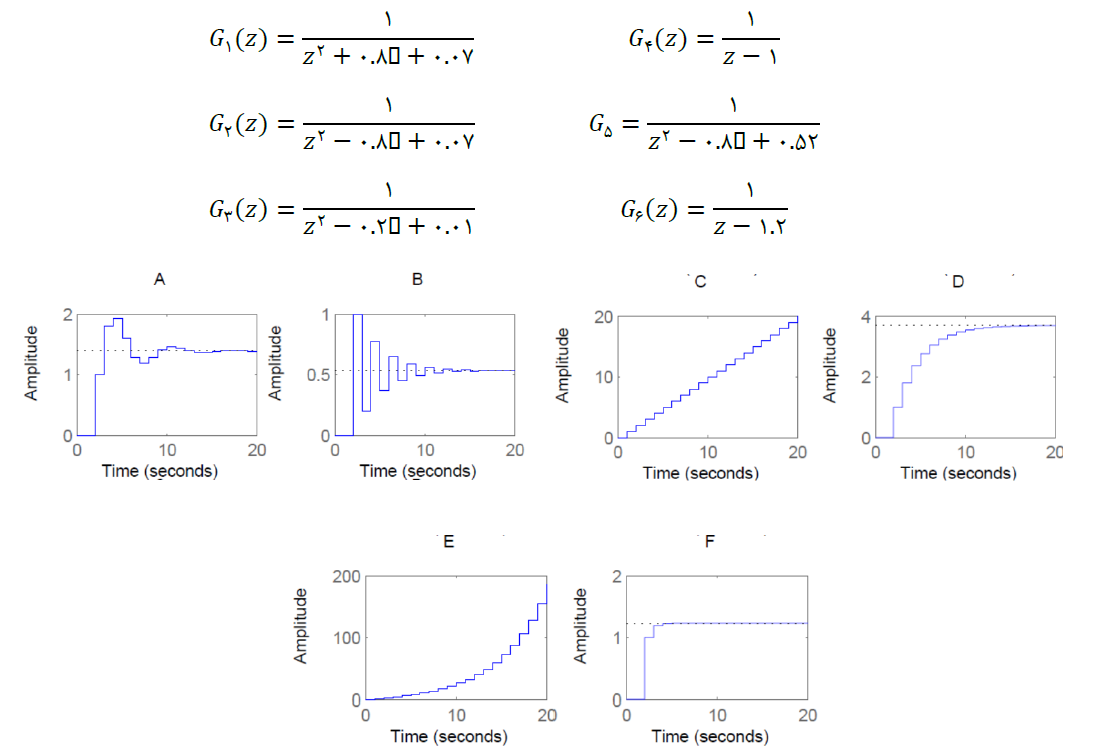
\includegraphics[width=\linewidth]{Second Series/1.png}
	\caption{شکل سوال یازدهم}
\end{figure}


\begin{problem}{سوال دوازدهم}
	(تبدیل ستاره) برای سیستم نمونه‌برداری شده شکل ذیل؛ تنها با استفاده از روش مدل گذر سیگنال 
	$C(s)$
	و
	$C(z)$
	را بیابید.

\end{problem}
\begin{figure}
	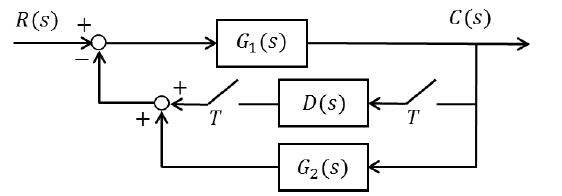
\includegraphics[width=\linewidth]{Second Series/6.png}
	\caption{شکل سوال دوازدهم}
\end{figure}


\begin{problem}{سوال سیزدهم}
	(تبدیل ستاره) مطلوبست
	$\frac{Y(z)}{R(z)}$
	و
	$\frac{Y(s)}{R^*(s)}$
	(در صورت وجود)
	
	
\end{problem}
\begin{figure}
	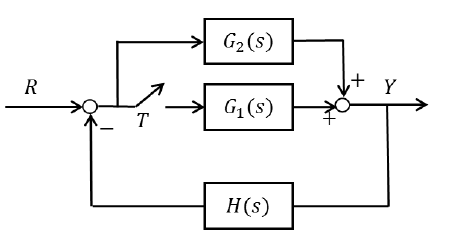
\includegraphics[width=\linewidth]{Second Series/7.png}
	\caption{شکل سوال سیزدهم}
\end{figure}

\begin{problem}{سوال چهاردهم}
	(تحقق) (میانترم 1401) تابع تبدیل $G(z)$ زیر را در نظر بگیرید.
	
	\centering
	$G(z) = \frac{z + 0.2}{(z-0.1)(z^2-0.5z+1)}$
	
	\raggedright
	الف) تحقق موازی سسیستم فوق را بدست آورید (برای بلوک های موازی از نحقق کنترل پذیر استفاده کنید.)
	
	ب) معادلات حالت سیستم را بدست آورید.
	
\end{problem}


\begin{problem}{سوال پانزدهم}
	(تبدیل $z$) تابع تبدیل ذیل را در نظر بگیرید: 
	
	\centering
	$G(s) = \frac{s+b}{s+a} , a > 0 , b <0$ 
	
	\raggedright
	این تابع تبدیل را با روش تبدیل $z$ استاندارد با پریود $T$ گسسته سازی نمایید. آیا تابع تبدیل گسسته نیز نامینیمم فاز خواهد بود؟ آیا
	پریود نمونه برداری وجود دارد که سیستم معادل گسسته مینیمم فاز باشد؟
\end{problem}


\end{document}
